\documentclass[a4paper]{article}

\usepackage[font=small,format=plain,labelfont=bf,up,textfont=up]{caption}
\usepackage[margin=2cm]{geometry}
\usepackage{graphicx}
\usepackage{minted}
\usepackage{todonotes}

\title{ELEC2221 D1: Design and test of a sequential multiplier}
\author{Kier Davis \\
Username: kad2g15 \\
Course: MEng Electronic Engineering \\
Tutor: Dr. Klaus-Peter Zauner \\
Lab group: F17 \\
Lab session: November 21, 2016}

\setminted{fontsize=\scriptsize,linenos}

\begin{document}

\maketitle

\begin{abstract}
  \todo[inline]{blah}
\end{abstract}

\section{Adder design, simulation and synthesis}
\label{sec:adder}

The adder was implemented as an integrated part of the \texttt{multiplier\_datapath} module.

\subsection{Implementation}
\label{sec:adder:impl}

The source code for the adder is given by lines 69--72 of Listing~\ref{lst:multiplier_datapath}.

\subsection{Simulation}
\label{sec:adder:sim}

The adder was not simulated on its own, but only as a part of \texttt{multiplier\_datapath} (see Section~\ref{sec:reg:sim}). \todo{finish}

\section{Register design, simulation and synthesis}
\label{seg:reg}

The registers were implemented in the \texttt{multiplier\_datapath} module, together with the adder/shifter.

The \texttt{multiplier\_datapath} module has two 4-bit data inputs, \texttt{multiplicand} and \texttt{multiplier}. These are the two input numbers to the multiplier, and are equivalent to \texttt{M} and \texttt{Qin} respectively in the sample code. Similarly, there is one 8-bit data output, \texttt{product}, which is equivalent to \texttt{AQ} in the sample code.

The module takes two control signals, \texttt{do\_init} and \texttt{do\_shift}, in addition to the clock and asynchronous reset signals. If \texttt{do\_init} is asserted during a rising clock edge, the \texttt{a} and \texttt{q} registers are loaded with their initial values (0 and \texttt{multiplier} respectively). If \texttt{do\_shift} is asserted during a rising clock edge, then \texttt{multiplicand} is conditionally added to \texttt{a}, and then \texttt{a} and \texttt{q} are shifted right by one place, completing one iteration of the multiplication algorithm in a single clock cycle.

\subsection{Implementation}
\label{sec:reg:impl}

The source code of the \texttt{multiplier\_datapath} module is given in Listing~\ref{lst:multiplier_datapath}.

\begin{listing}[ht]
  \inputminted{systemverilog}{../src/multiplier/multiplier_datapath.sv}
  \centering\caption{Source code of the \texttt{multiplier\_datapath} module, which contains the data registers $a$ and $q$ and the add/shift computation logic.}
  \label{lst:multiplier_datapath}
\end{listing}

\subsection{Simulation}
\label{sec:reg:sim}

A testbench for the \texttt{multiplier\_datapath} module was prepared. Its source code is given in Listing~\ref{lst:test_multiplier_datapath}. The testbench was then simulated using ModelSim, giving the waveform diagram shown in Figure~\ref{fig:test_multiplier_datapath}. After correcting some minor syntax errors, the testbench and the module under test worked first time, without any assertions failing.

The testbench begins with the reset signal active, and checks that the registers \texttt{a} and \texttt{q} (whose values are concatenated to form the signal \texttt{product}) are reset to zero. It then releases the system from reset, and asserts the \texttt{do\_init} for one clock cycle, checking that \texttt{q} is set to 6, the value arbitrarily chosen for the second multiplier input. It then asserts \texttt{do\_shift} for four of the five following clock cycles, checking the state of the registers at each stage. The results of these operations can be observed in Figure~\ref{fig:test_multiplier_datapath}.

\begin{listing}[ht]
  \inputminted{systemverilog}{../src/multiplier/test/test_multiplier_datapath.sv}
  \centering\caption{Source code of the \texttt{test\_multiplier\_datapath} module, which tests the operation of the data registers and add/shift computation logic.}
  \label{lst:test_multiplier_datapath}
\end{listing}

\begin{figure}[ht]
  \centering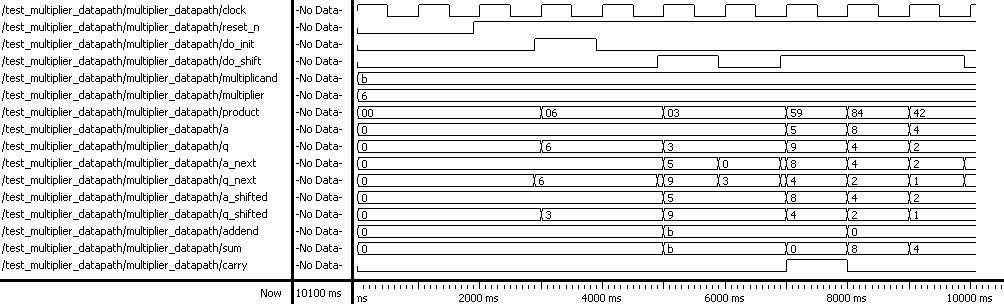
\includegraphics[width=\textwidth]{assets/test_multiplier_datapath}
  \centering\caption{Waveform of the \texttt{test\_multiplier\_datapath} testbench.}
  \label{fig:test_multiplier_datapath}
\end{figure}

\section{Sequencer design, simulation and synthesis}
\label{sec:seq}

\todo[inline]{todo}

\subsection{Implementation}
\label{sec:seq:impl}

The 2-bit counter used for counting the number of remaining iterations of the shift/add operation is implemented in the \texttt{multiplier\_counter} module, whose source code is given in Listing~\ref{lst:multiplier_counter}. The remainder of the state machine is implemented in the \texttt{multiplier\_controller} module, whose source code is given in Listing~\ref{lst:multiplier_controller}.

\begin{listing}[ht]
  \inputminted{systemverilog}{../src/multiplier/multiplier_counter.sv}
  \centering\caption{Source code of the \texttt{multiplier\_counter} module, which contains the 2-bit counter that records the number of remaining iterations of the algorithm.}
  \label{lst:multiplier_counter}
\end{listing}

\begin{listing}[ht]
  \inputminted{systemverilog}{../src/multiplier/multiplier_controller.sv}
  \centering\caption{Source code of the \texttt{multiplier\_controller} module, which contains the state machine that controls the multiplier's operation.}
  \label{lst:multiplier_controller}
\end{listing}

\subsection{Simulation}
\label{sec:seq:sim}

\todo[inline]{todo}

\section{Multiplier design, simulation and synthesis}
\label{sec:mult}

\todo[inline]{todo}

\subsection{Implementation}
\label{sec:mult:impl}

The encapsulating module is named \texttt{multiplier}, and consists of the source code given in Listing~\ref{lst:multiplier}. Also, Listing~\ref{lst:frontend}.

\begin{listing}[ht]
  \inputminted{systemverilog}{../src/multiplier/multiplier.sv}
  \centering\caption{Source code of the encapsulating module \texttt{multiplier}.}
  \label{lst:multiplier}
\end{listing}

\begin{listing}[ht]
  \inputminted{systemverilog}{../src/frontends/machxo2_pico_frontend.sv}
  \centering\caption{Source code of the MachXO2 Pico frontend module \texttt{machxo2\_pico\_frontend}.}
  \label{lst:frontend}
\end{listing}

\subsection{Simulation}
\label{sec:mult:sim}

\todo[inline]{todo}



\end{document}
